\documentclass{article}
\usepackage{graphicx}
\usepackage{hyperref}

\begin{document}

\title{The HypeDyn Hypertext Fiction Editor\\Tutorial 2: Links with Multiple
Rules, Conditional Text and Anywhere Nodes}
% \author{Alex Mitchell}
\date{}

\onecolumn
\maketitle

\tableofcontents


\section{Introduction}
In this tutorial, we will introduce some new features to HypeDyn:

\begin{itemize}
  \item links with \textit{multiple rules}, which allows for different actions
  to be taken depending on which conditions are satisfied;
  \item \textit{conditional text}, which can be displayed \textit{instead of}
  the original text in a link; and \item \textit{anywhere nodes}, which are
  nodes that can be linked to from any other nodes in the story based on
  conditions.
\end{itemize}

In this tutorial, we will be creating a variation of the ``Little Red Riding
Hood'' hypertext fiction which you created in tutorial 1. We will change the
story such that the reader is able to choose whether Red is naive or
street-smart, which will have consequences as to how the story ends, and will
also cause some of the text in the story to change. We will also add a
``summary'' node, reachable from all other nodes, which shows an up-to-date
summary of the story so far.

\begin{figure}[h]
  \centering
  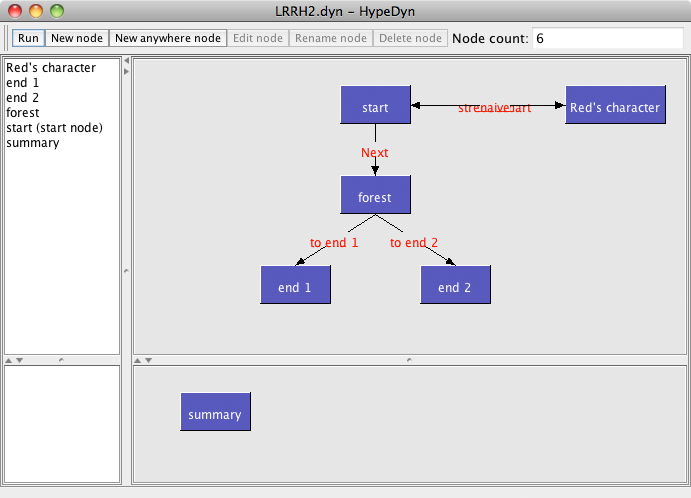
\includegraphics[width=11cm]{images/hypedyn-tutorial-2-figure-1}
  \caption{\textit{The completed ``Little Red Riding Hood'' story.}}
  \label{fig:tut2:completed}
\end{figure} 

The nodes and links in the final story are shown in Figure \ref{fig:tut2:completed}.

\textit{Note:  HypeDyn is a work-in-progress. If you encounter any errors, please
report them as bugs on our Launchpad site: \url{https://launchpad.net/hypedyn}.}

\section{Getting started}

First, open HypeDyn by double-clicking on the file \textbf{HypeDyn.exe} (in
Windows) or \textbf{HypeDyn.app} (in MacOS).

We will continue from the story that you created in tutorial 1. If you don't
have the story, you can start from the file \textsc{LRRH.dyn} in the
\textsc{examples} folder. HypeDyn files always end with a \textbf{.dyn} extension.

% \textit{Note: for users of Ariadne, the HypeDyn file format is different
% from the Ariadne file format. If you have your LRRH.xml file from the Ariadne tutorial,
% you will not be able to load it in HypeDyn.}

We no longer need the ``Hood details'' node, so delete this node by clicking on
the node in either the node list on the left of the main window, or in the
map view on the right of the main window, and then clicking the ``Delete node''
button. Then go into the ``start'' node, and delete the link ``more about
the hood'' which previously led to the ``Hood details'' node. Save the resulting
file under a different name.

% also need to delete the link, and the ``restart'' link and text in end node

\section{Links with multiple rules}

The first new feature we will introduce is the use of multiple rules on a link.
This feature allows you to have different sets of actions which will be
triggered when different conditions are satisfied.

For our story, we want to provide two different endings: one ending if Red is
naive, and a second ending if she is street-smart. We will provide one link for
the reader to click on and, depending on the choice that the reader made at the
start of the story, the link will lead to either the first or the second ending.

\subsection{Letting the reader make a choice}

To let the reader make a choice, we will create a node named ``Red's character'',
which contains two links, one named ``naive'' and another named ``street-smart''.
Both links lead back to the start node. HypeDyn will keep track of which link was
followed. Later in the story, we can check which of these two links the reader
chose, and use this to make a decision. We will do this by creating a rule on the
``to the end'' link in the ``forest'' node which leads to node ``end1'' if link
``naive'' was followed, and a second rule which goes to node ``end2'' if link
``street-smart'' was followed.

Now we will create the node ``Red's character'' to let the reader make a
choice.

\begin{enumerate}
  \item Create a new node named ``Red's character''. In the new node, enter the
following text:

\begin{quotation}
\noindent Is Red naive or street-smart?
\end{quotation}

\item Make a link on the text ``naive''.

\item Create one rule in the link, and also name the rule ``naive''.

\item Recall that the \textit{Edit rule} dialogue contains a list of conditions
(initially empty), plus a list of actions. The actions will be performed if the
rule defined by the conditions is satisfied.

Since we don't want the reader to be able to change their choice, we will put a
condition on this link: the link can only be followed if the reader
\textit{hasn't} followed both the link ``naive'' and the link ``street-smart''.
Do this by adding 2 conditions to the rule, as shown in Figure
\ref{fig:tut2:red_is_naive}.

\begin{figure}[h]
  \centering
  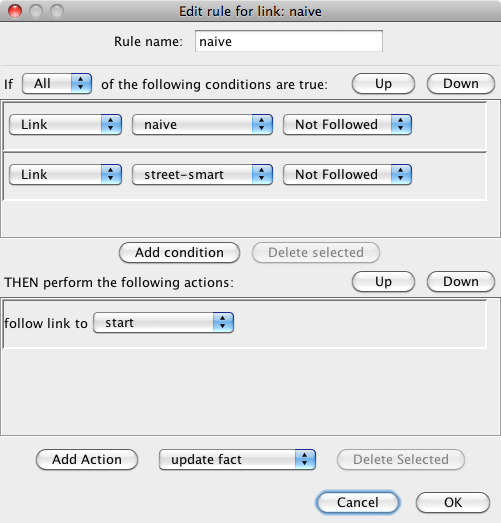
\includegraphics[width=9cm]{images/hypedyn-tutorial-2-figure-2}
  \caption{\textit{Adding conditions on the link to ``Red is naive''.}}
  \label{fig:tut2:red_is_naive}
\end{figure} 

\noindent In Tutorial 1, we used conditions which checked whether or not a
\textit{node} had been \textit{visited}. Here, we are using conditions which
check whether or not a \textit{link} has been \textit{followed}. HypeDyn also
provides conditions which can check the state of \textit{facts}. We will cover
facts in Tutorial 3.

\item Do the same to create a link from the text ``street-smart'' to the
``start'' node, with the same conditions as the ``naive'' link.

\item Finally, edit the node ``start'', and make a link from the text ``Little
Red Riding Hood'' to the node ``Red's character''. Name the link ``Red's
character''. We don't want the reader to be able to go into ``Red's Character''
if they have already made a choice, so create the same conditions on this link
as you did on ``naive'' and ``street-smart''.

\noindent Note that even though we put this condition on the link to ``Red's
character'', we still need the conditions on the two links in the ``Red's
character'' node, just in case the reader presses the ``back'' button and
tries to change their choice. Also, we can't just check whether or not the
reader has visited the node ``Red's character'', as they may not have actually
made a choice.
\end{enumerate}

Now we have the mechanism in place to let the reader choose what sort of person
Red is: naive or street-smart. Now we can check which of the two links were
followed, ``naive'' or ``street-smart'', whenever we want to make a decision
which is influenced by Red's character. This is an example of using the
\textit{followed state} of a link as a way of representing some information about
the state of the storyworld. Similarly, we could use the \textit{visited state}
of a node to represent some information. This is a very useful technique which
can be generalized to allow for more complex, dynamic behaviour.

% bug!!! ``Red's character'' link not displayed correctly at first

\subsection{Following a link based on the reader's choice}

Now we will create the link to the two different endings, and set up the rules so
that the reader will follow the link to the appropriate ending based on the
reader's earlier choice about Red's character.

\begin{enumerate}
  \item First, rename the current ``end'' node to ``end 1'' by selecting the
  node in the map view, and clicking on the ``Rename node'' button. Type in the
  new name, and click ``Ok''.
  \item Edit the node ``end 1'', and delete the text ``back to start''. Notice
  that the link to the ``start'' node is deleted when you delete the text.
  \item Next, replace the text in the node ``end 1'' with the following text:
  \begin{quotation}
  \noindent Quickly the wolf ran ahead to Grandma's house, swallowed Grandma
  whole, and disguised himself as the poor old lady. When Red arrived, he finished her
  off too. Yum!
  
  \bigskip
  
  \noindent *** The End ***
  \end{quotation}
  \item Now create a new node, named ``end 2'', and enter the following text:
  \begin{quotation}
  \noindent Frustrated, the wolf snuck off to try his luck at the mall instead.
  
  \bigskip
  
  \noindent *** The End ***
  \end{quotation}

\item Now that we have the two endings in place, we need to make sure that the
link from the text ``next'' in node ``forest'' takes the reader to ``end 1'' if Red
is naive. Otherwise (ie. if Red is street-smart), the link should take the
reader to ``end 2''. To do this, we will add conditions to the current rule,
and then add a second rule to the ``to the end'' link.

Edit the ``to the end'' link on the text ``next'' in node ``forest''.
The original link, from the previous version of the story, has a single rule,
``to the end'', which has no conditions and contains a single ``follow link
to'' action, leading ot the original end node, now renamed ``end 1''.

\item We are doing to change this rule so that it only takes the reader to
``end 1'' if Red is naive. To help us remember this, we can rename the rule to
reflect what it does. Rename the rule as ``to end 1''. This is the label which
will appear in the map view.

\item Now add a condition that link ``naive'' is followed (see Figure
\ref{fig:tut2:to_end_1}).

\begin{figure}[h]
  \centering
  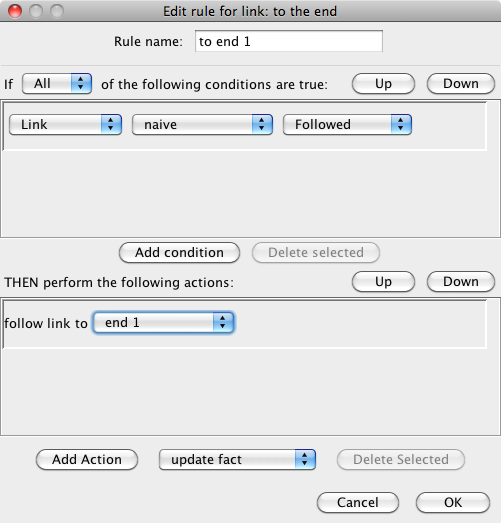
\includegraphics[width=9cm]{images/hypedyn-tutorial-2-figure-3}
  \caption{\textit{Condition on the rule leading to ``end 1''.}}
  \label{fig:tut2:to_end_1}
\end{figure}

\item This gives us the required behaviour for a naive Red. However, if the
conditions are \textit{not} satisfied, ie. if Red is street-smart, the link
won't go anywhere. Next we need to use the same link, but now specify what
should happen in this case. To do this, we will create a second rule.

Exit the \textit{Edit rule} dialog by clicking on ``Ok''. You should now be at
the \textit{Edit link} dialog, which contains one rule (see Figure
\ref{fig:tut2:rules_before}).

\begin{figure}[h]
  \centering
  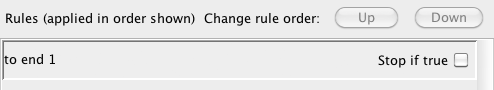
\includegraphics[width=9cm]{images/hypedyn-tutorial-2-figure-4}
  \caption{\textit{One rule leading to ``end 1''.}}
  \label{fig:tut2:rules_before}
\end{figure}

\item Add a second rule by clicking on the ``Add Rule'' button. You should now
see a second rule beneath the ``to end 1'' rule, named ``new rule''.

\item Now edit the new rule by selecting the rule and clicking on the ``Edit
Rule'' button.

\item Change the name of the rule to ``to end 2''. This will remind us that
this rule contains the action to follow the link to ``end 2''.

\item Add a ``follow link to'' action, and set its pulldown menu to ``end 2''.

\item Close the \textit{Edit rule} dialog by clicking on the ``Ok'' button. You
will be taken back to the \textit{Edit link} dialog, where you should see 2
rules: ``to end 1'' and ``to end 2'' (see Figure \ref{fig:tut2:rules_with_new}).

\begin{figure}[h]
  \centering
  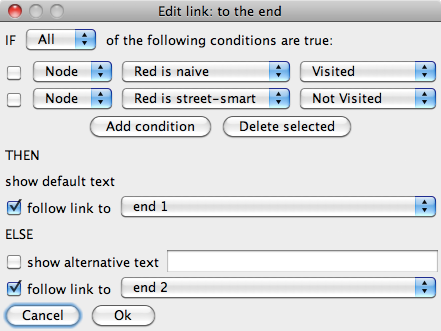
\includegraphics[width=9cm]{images/hypedyn-tutorial-2-figure-5}
  \caption{\textit{Adding a second rule.}}
  \label{fig:tut2:rules_with_new}
\end{figure}

\item At this point, we have two rules, one which leads to ``end 1'' if the
link ``naive'' was followed, and the other which always leads to ``end 2''.
This is not quite right -- what will happen if you try reading the story now?
First try choosing Red's character to be naive, and then restart the story and
try making her street-smart.

As you will have noticed, the link always goes to ``end 2'', whichever link you
choose in ``Red's character''. To understand why this is, we need to look at
how HypeDyn evaluates rules.

When the reader clicks on a link, HypeDyn looks at the rules in a link one by
one, from the top of the list of rules. For each rule, it determines whether the
conditions are satisfied. If the conditions are \textit{not} satisfied, it goes
to the next rule, and again checks this rule's conditions. It keeps doing this
until it finds a rule for which the conditions are satisfied. Once this happens,
it carries out the actions in that rule.

After the actions have been carried out, HypeDyn looks to see whether or not the
``Stop if true'' option has been checked for the current rule. If it has been
checked, then it stops. Otherwise, it continues on to the next rule, and
repeats the process of checking conditions and carrying out actions.

So in our case, HypeDyn first looks at the ``to end 1'' rule. In the case where
the reader has chosen ``street-smart'', HypeDyn will check the conditions for
``to end 1'', see that they are not satisfied, and then move on to the second
rule. Since there are no conditions on the second rule, HypeDyn carries out its
actions, taking the reader to node ``end 2''. This is what we want.

If the ``naive'' link has been followed, HypeDyn checks the conditions for the
``to end 1'' rule, sees that they \textit{are} satisfies, and carries out the
action, taking the reader to node ``end 1''. It then looks at the ``Stop if
true'' option, which is not checked, and moves on to the second rule, ``to end
2''. Since there are no conditions on the second rule, HypeDyn carries out its
actions, taking the reader to node ``end 2''. This is \textit{not} what we want!

\item To fix this, the easiest solution is to check the ``Stop if true'' option
on the ``to end 1'' rule. This will tell HypeDyn not to continue to the next rule
if the first rule has been satisfied. Do this now (see Figure
\ref{fig:tut2:rules_with_stop}).

\begin{figure}[h]
  \centering
  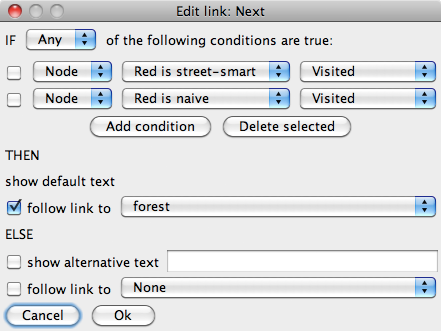
\includegraphics[width=9cm]{images/hypedyn-tutorial-2-figure-6}
  \caption{\textit{Stopping if the first rule is satisfied.}}
  \label{fig:tut2:rules_with_stop}
\end{figure}\item 

Now try running the story again. It should behave as we intended -- if the
we choose that Red is naive, we will see the first ending, and if we choose
that she is street-smart, we will see the second ending.

\end{enumerate}

Note that there is another way to fix this problem. Instead of checking the
``Stop if true'' option on the ``to end 1'' rule, we could have put a condition
on the ``to end 2'' rule stating that the rule's actions should only be carried
out if the ``street-smart'' link was followed. However, this would mean that
every time the reader chooses the ``naive'' link, the second rule's conditions
are checked. For such a simple rule this is not a problem, but if the rule
becomes more complex, this can slow down your story.

\subsection{Forcing the reader to make a choice}

At this point we seem to have everything in place for the reader to make a
choice which impacts the end of the story. However, with our current
implementation, if the reader ignores the link on the text ``Little Red Riding
Hood'' in the ``start'' node, and goes through to the end of the story, she will
always end up with the second ending.

To fix this, we need to force the reader to make the choice about Red's character
\textit{before} we let her move on to the ``forest'' node. We can do this by
putting a condition on the link from ``start'' to ``forest'' such that the link
can only be followed if \textit{either} link ``naive'' \textit{or} link
``street-smart'' have been followed.

% bug!!! link can't be followed - link followed not updated at the correct time?

\begin{enumerate}
  \item Edit the rule ``Next'' in the link ``Next'' in node ``start''.
  \item Add the following condition: link ``naive'' was followed.
  \item Add the following condition: link ``street-smart'' was followed.
  \item Now change the pulldown menu to the right of ``IF'' to show ``Any'' (see
  Figure \ref{fig:tut2:any_condition}).

\begin{figure}[h]
  \centering
  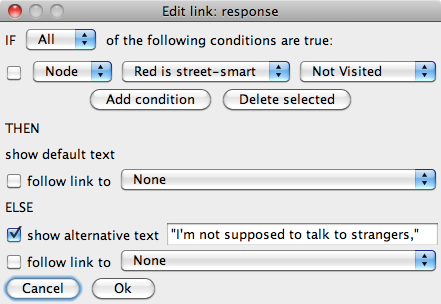
\includegraphics[width=9cm]{images/hypedyn-tutorial-2-figure-7}
  \caption{\textit{Specifying two conditions where \textbf{any} can be
  satisfied.}}
  \label{fig:tut2:any_condition}
\end{figure} 

This means that the link will be followed if \textit{any} of the listed
conditions are satisfied, which is what we want.

\end{enumerate}

\subsection{Testing the story}

Now that we have our story in place, we can test the story. You can do this by
clicking the ``Run'' button. The ``Run'' button will read the story starting at
the node which was set as the \textit{start} node, which will be indicated by the
text ``(start)'' to the right of the node name in the node list.

Try clicking through the story. You should be able to choose Red's character, and
then see a different ending based on your choice. You can stop reading by closing
the ``Reader'' window in your browser.

\section{Specifying conditional text}

As you read through the story, you probably realized that there's a problem:
the story doesn't really make sense. There's no explanation as to why the wolf
was unable to eat Red if she's street-smart. It also doesn't seem reasonable
that, as a street-smart little girl, she would have told the wolf that she was
going to Grandma's house.

So, it would be good if we could change what Red says to the wolf depending on
what choice the reader made regarding Red's character. This is where
\textit{conditional text} is useful.

What we want to do is set a condition so that, if the reader has chosen for
Red to be street-smart, the text ``I'm off to see my sick granny'' in the
``forest'' node will automatically be changed to ``I'm not supposed to talk to
strangers.''

\begin{enumerate}
  \item Edit the node ``forest''.
  \item Select the text ``I'm off to see my sick granny'', and click on
  ``New link''.
  \item In the ``New link" dialogue, name the link ``response'', and click
  ``ok''. You should see the ``Edit link'' dialogue.
  \item In the ``Edit link'' dialogue, create a new rule.
  \item Edit the new rule, and rename it ``street-smart''.
  \item Add a condition, and set the following condition: link ``street-smart''
  is followed.
  \item Now add an ``update text using'' action. Make sure the action's
  pulldown menu reads ``alternative text'', and type the following text into
  the action's text field (see Figure \ref{fig:tut2:alttext}):
  \begin{quotation}
  \noindent ``I'm not supposed to talk to strangers.''
  \end{quotation}

\begin{figure}[h]
  \centering
  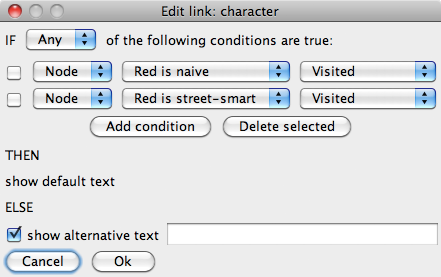
\includegraphics[width=9cm]{images/hypedyn-tutorial-2-figure-8}
  \caption{\textit{Specifying alternative text.}}
  \label{fig:tut2:alttext}
\end{figure} 

  Since we don't want the reader to actually be able to click on this
  link, we won't add a ``follow link to'' action. Without a ``follow link to''
  action, the link will not be underlined or bold.
  \item Click on ``ok'' to close the ``Edit rule'' dialog, and then on the
  ``Close'' button to close the ``Edit link'' dialog.
%   Note that the node
%   as displayed in the map view is now shown as a ``stack'' of nodes - this is
%   to remind you that you've created conditional text on this node.
\end{enumerate}

That's it! Now test the story by clicking on the ``Run'' button. You should see
the appropriate text in the ``forest'' node, depending on which personality you
chose for Red.

This is a simple feature, but it is a major addition to what can be done in
HypeDyn. Text is no longer fixed - the author can procedurally alter/generate
text within a node, based on the reader's actions. 

Note that we could get the same effect (from the reader's perspective) by
creating 2 nodes -- one with the original text, and one with the ``street-smart''
text. This is a reasonable solution when there is one change, such as in our
simple story for this tutorial. However, if there are many nodes which need to
be changed based on the choice of Red's character, it will quickly become
difficult for the author to keep track of the text. It gets even more
complicated if there are more than one choices which the reader can make. Using
conditional text is a much more appropriate and manageable approach.

\section{Anywhere nodes}

The last thing we are going to do is to add in an ``anywhere'' node. This is a
node which is automatically linked from all the nodes in the story. This
feature is useful as a way to create, for example, a summary of the story so
far, or a list of the decisions that the reader has made. 

\subsection{Adding the anywhere node}
In our case, we will create a summary of the story so far using an anywhere
node.

\begin{enumerate}
  \item Click on ``New anywhere node'', and name the new node ``summary''.
  Notice that the new node is a darker grey that regular nodes. The difference
  in colour is used to indicate anywhere nodes. Note that an anywhere node is 
  almost the same as a regular node, with the exception of a special action that
  is added automatically to the ``node rules''. Removing this action turns an
  anywhere node into a regular node. We will discuss node rules in Tutorial 3.

  \item Edit the node by selecting it and clicking on ``Edit node'', as with a
  regular node.

  \item In the node, enter the following text:
  \begin{quotation}
  \noindent The story has begun.
  
  \bigskip
  
  \noindent Red's character has been decided.

  \bigskip

  \noindent Red has met the wolf.

  \bigskip

  \noindent The end.
  \end{quotation}
\end{enumerate}

If you run the story now, you will see a link with the text ``summary'' has
been added to the bottom of every node. Clicking on this link will take you to
the node which we just created.

\subsection{Adding some conditional text}
We want the second line to be displayed only after the reader has decided on
Red's character, the third line after the ``forest'' node has been visited, and
the last line once the reader has reached the end of the story. We can do this
using conditional text, as shown in the previous section.

\begin{enumerate}
  \item Select the second line of text, and click on ``New link''. Name the link
  ``character'' and click ``ok''.
  \item Create a new rule, edit the rule, and also name it ``character''.
  \item We want the text under this link to only be shown after the reader has
  decided on Red's character. So first what we need to do is create an action
  to \textit{remove} the text. Add an ``update text using'' action, and leave
  the text blank. This will blank out the link text when this rule's conditions
  are met.
  
  \item Now we want to set the conditions for when the text is blanked. Since we
  want the first line to show after the reader has chosen Red's character, we
  need two conditions: the link ``naive'' has \textit{not} been followed,
  and the link ``street-smart'' has \textit{not} been followed. Add these two
  conditions.
  \item Since we want the text to show when both of these links have not been
  followed, make sure the the type of the rule is set to ``All''.
\item Click ``Ok'' to close the ``Edit rule'' dialog, and then close the ``Edit
link'' dialog.
\end{enumerate}

\subsection{Adding the remaining conditional text}
Now do the same for the third and final lines:

\begin{enumerate}
  \item Add a link, named ``forest'', on the third line.
  \item Add a rule, also named ``forest'', to the ``forest'' link.
  \item Add one condition, that the ``forest'' node has not been visited.
  \item Add an ``update text using'' action, leave the text blank, then click
  ``Ok'', and close the ``Edit link'' dialog.
  \item Add a link, named ``end'', on the final line.
  \item Create a rule, and also name it ``end''.
  \item Add two conditions, that the ``end 1'' node has \textit{not} been
  visited, and that the ``end 2'' node has \textit{not} been visited.
  \item Finally, add an ``update text using'' action, leave the text blank,
  then click ``Ok'', and close the ``Edit link'' dialog.
\end{enumerate}

This completes the ``summary'' node. Try running the story, and go through
the two story. There should now be a ``summary'' link at the bottom of all
regular nodes. If you click on the link, you should see a node with the summary
of the story. The text in the summary node should gradually be revealed as you
move through the story.

\section{Next steps}

We have created a simple story, with a choice at the start which changes what
happens in the story, including the ending. The completed version of this story
can be found in the file \textsc{LRRH2.dyn}.

There are several things that you could try to enhance the story. For example,
you could change the description of Red in the ``start'' node, depending on
whether she is naive or street-smart. You could also customize the summary of
the story depending on which personality the reader chose. One way of adding
these enhancements can be found in \textsc{LRRH3.dyn}.

\section{Conclusion}

In this tutorial, we have created a simple hypertext fiction which includes a
choice for the reader regarding Red Riding Hood's character. We have seen how to
make use of multiple rules and conditional text to adapt the story to the
reader's choice. This funcitonality provides the basis for moving away from
stories which make use of predetermined content and branches, towards more
procedural hypertext. In tutorial 3, we explore more extensive use of procedural
hypertext, introducing ``node rules'' and ``facts''.

\end{document}
